% ============================================================================
% Artigo de TCC — formato SBC, citações e referências em conformidade com a
% ABNT (NBR 10520:2023 para citações, NBR 6023:2018 para a lista de
% referências, ao final do arquivo).
% ============================================================================

\documentclass[12pt]{article}

\usepackage{sbc-template}
\usepackage{graphicx,url}
\usepackage{placeins}
\usepackage[utf8]{inputenc}
\usepackage[T1]{fontenc}
\usepackage[provide=*,brazilian]{babel}

\sloppy

\title{Um Aplicativo Móvel para Gerenciamento de Treinos com Detecção da Qualidade de Execução de Exercícios via Visão Computacional}

\author{Fernando Bordin Correa\inst{1}}

\address{{Engenharia da Computação} -- {PUC Campinas}\\
  {Campinas} -- Brasil
  \email{fernando.bordin.correa@gmail.com}
  \\\mbox{}\\[-6pt]\footnotesize Orientador(a): Antonio Paulo Salgado Forster
}

\begin{document}

\maketitle

\begin{abstract}
  Incorrect execution of resistance-training exercises is a common cause of
  injury and reduced training effectiveness, and beginners rarely have
  access to a professional supervising every repetition. This work presents
  a mobile application for workout planning and logging that also detects,
  from a smartphone camera, whether a given repetition of an exercise was
  performed correctly. The system combines pose estimation (MediaPipe Pose)
  with a per-exercise supervised classifier (Random Forest or SVM,
  selected by cross-validation) trained on joint angles extracted at the
  peak of each repetition. We describe the system's architecture (React
  Native/Expo client, FastAPI backend, PostgreSQL/SQLite persistence),
  the video-analysis pipeline used for classification, the cloud deployment
  on Microsoft Azure, and a training-dataset coverage gap for high-amplitude
  repetitions found along the way.
\end{abstract}

\begin{resumo}
  A execução incorreta de exercícios de musculação é uma causa comum de
  lesões e de baixa efetividade do treino, e iniciantes raramente têm
  acesso a um profissional supervisionando cada repetição. Este trabalho
  apresenta um aplicativo móvel de planejamento e registro de treinos que
  também detecta, a partir da câmera do celular, se uma repetição de um
  exercício foi executada corretamente. O sistema combina estimativa de
  pose (MediaPipe Pose) com um classificador supervisionado por exercício
  (Random Forest ou SVM, escolhido por validação cruzada) treinado sobre
  ângulos articulares extraídos no pico de cada repetição. Descrevemos a
  arquitetura do sistema (cliente React Native/Expo, backend FastAPI,
  persistência em PostgreSQL/SQLite), o pipeline de análise de vídeo usado
  na classificação, a implantação em nuvem na Microsoft Azure e uma lacuna
  de cobertura do dataset de treino para repetições de amplitude elevada,
  encontrada ao longo do desenvolvimento.
\end{resumo}

\section{Introdução}

A prática regular de exercícios resistidos (musculação) é amplamente
recomendada por seus benefícios à saúde física e mental
\cite{worldhealth2020}. No entanto, a efetividade e a segurança desse tipo
de treino dependem fortemente da qualidade da execução: repetições
realizadas com amplitude, ângulo articular ou controle inadequados reduzem
o estímulo ao músculo-alvo e aumentam o risco de lesão. Praticantes
iniciantes, em especial os que treinam sem acompanhamento de um
profissional de educação física, não têm como avaliar objetivamente se
estão executando um movimento corretamente, dependendo de autoavaliação ou
de vídeos genéricos que não analisam a execução específica do usuário.

Ao mesmo tempo, a popularização de \textit{smartphones} com câmeras de boa
qualidade e o amadurecimento de bibliotecas de estimativa de pose humana em
tempo real, como o MediaPipe Pose \cite{lugaresi2019mediapipe,
bazarevsky2020blazepose}, tornaram viável construir sistemas de análise de
movimento que rodam com hardware acessível, sem depender de sensores
vestíveis ou de múltiplas câmeras calibradas.

Este trabalho descreve o desenvolvimento de um aplicativo móvel de
gerenciamento de treinos -- com cadastro de exercícios, montagem de fichas
de treino e registro de sessões -- que incorpora um
\textit{detector} de execução de exercícios: o usuário grava (ou envia) um
vídeo de si mesmo executando um exercício e o sistema retorna, repetição a
repetição, se a execução foi classificada como correta ou incorreta.

\subsection{Objetivos}

O objetivo geral deste trabalho é desenvolver e avaliar um sistema mobile
completo de apoio ao treino de musculação, com um módulo de detecção
automática da qualidade de execução de exercícios baseado em visão
computacional. Como objetivos específicos, destacam-se:

\begin{itemize}
  \item Implementar um aplicativo móvel para Android, sobre uma stack
  multiplataforma (React Native/Expo), para planejamento, execução e
  histórico de treinos;
  \item Desenvolver um backend que centralize a persistência de dados dos
  usuários, treinos e sessões, e que hospede o serviço de análise de vídeo;
  \item Construir um pipeline de extração de características a partir de
  pose humana e um classificador capaz de distinguir repetições corretas de
  incorretas para mais de um exercício;
  \item Implantar o sistema em um ambiente de nuvem, validando seu
  funcionamento fora do ambiente de desenvolvimento local;
  \item Identificar e documentar as limitações do modelo de detecção
  atual, propondo direções para superá-las.
\end{itemize}

O restante deste artigo está organizado da seguinte forma: a Seção~2
apresenta a revisão tecnológica; a Seção~3 apresenta a arquitetura geral do
sistema; a Seção~4 detalha o módulo de detecção de execução de exercícios;
a Seção~5 descreve a implantação em nuvem; a Seção~6 descreve a
metodologia de avaliação dos classificadores; a Seção~7 apresenta
resultados e limitações identificadas; e a Seção~8 conclui o trabalho e
aponta direções futuras.

\section{Revisão Tecnológica}

\subsection{Avaliação de Qualidade de Execução com Sensores Inerciais}

Velloso et al.~\cite{velloso2013hars} propuseram um dos primeiros trabalhos
a tratar explicitamente a \textit{qualidade} de execução de um exercício de
musculação -- e não apenas o reconhecimento de \textit{qual} exercício está
sendo realizado -- como um problema de classificação supervisionada. No
estudo, quatro unidades de medição inercial (\textit{IMU}) de 9 graus de
liberdade, cada uma combinando acelerômetro, giroscópio e magnetômetro
triaxiais e amostrando a 45\,Hz, foram fixadas em uma luva, um bracelete, um
cinto lombar e no próprio halter, capturando ângulos de Euler e as leituras
brutas dos três sensores em cada ponto. Participantes executaram repetições
de rosca bíceps unilateral (\textit{Unilateral Dumbbell Biceps Curl}) de
cinco formas diferentes, definindo cinco classes: execução correta segundo a
especificação (Classe A) e quatro erros comuns -- jogar os cotovelos para a
frente (Classe B), levantar o halter só até a metade do percurso (Classe C),
descer o halter só até a metade (Classe D) e jogar o quadril para a frente
(Classe E). Um classificador Random Forest, treinado sobre características
estatísticas extraídas em janelas deslizantes dos sinais dos quatro
sensores, atingiu 98,03\% de acurácia em validação cruzada 10-fold -- taxa
sensivelmente mais alta que a obtida pelos classificadores geométricos por
quadro deste trabalho (Seção~7), o que é esperado, já que sensores
inerciais captam diretamente grandezas físicas (aceleração, rotação) que uma
câmera só pode estimar indiretamente a partir da projeção 2D do corpo. Essa
mesma vantagem é, porém, sua principal limitação prática: cada sessão de
treino exige instrumentar o usuário com múltiplos sensores vestíveis fixados
em pontos específicos do corpo e do equipamento, o que inviabiliza o uso
espontâneo em uma academia comum -- restrição que abordagens baseadas em
visão computacional, discutidas a seguir, eliminam ao dispensar qualquer
instrumentação além de uma câmera comum.

\subsection{Estimativa de Pose Humana a partir de Vídeo}

A estimativa de pose humana busca localizar, a partir de uma imagem ou
vídeo comum, as coordenadas de um conjunto pré-definido de articulações do
corpo (\textit{landmarks}), sem exigir sensores ou marcadores físicos. As
abordagens se dividem, quanto à estratégia de detecção, em \textit{top-down}
e \textit{bottom-up}: métodos \textit{top-down} primeiro detectam cada
pessoa na imagem com um detector de objetos genérico e depois estimam a pose
de cada uma isoladamente, o que tende a preservar acurácia mas faz o tempo
de execução crescer com o número de pessoas na cena; métodos
\textit{bottom-up}, como o OpenPose, detectam todas as partes do corpo
presentes na imagem de uma só vez e só depois as associam aos indivíduos
correspondentes, mantendo tempo de execução praticamente constante
independentemente de quantas pessoas aparecem. Quanto à saída, a estimativa
pode ser 2D (coordenadas no plano da imagem, usada neste trabalho) ou 3D
(coordenadas com profundidade estimada, tipicamente mais custosa e
dependente de calibração ou de múltiplas vistas).

O OpenPose~\cite{cao2021openpose} é o representante mais estabelecido da
abordagem \textit{bottom-up}: emprega \textit{Part Affinity Fields}, uma
representação vetorial não paramétrica que codifica a posição e orientação
dos membros do corpo, para associar as partes detectadas aos indivíduos
corretos mesmo em cenas com múltiplas pessoas. Seu modelo original, treinado
sobre o dataset COCO, estima 18 pontos-chave do corpo (formato
\texttt{BODY\_18}); uma extensão posterior adiciona pontos do pé,
totalizando 25 pontos-chave (formato \texttt{BODY\_25}). O dataset
reaproveitado neste trabalho (Seção~2.3) foi gerado com o modelo original de
18 pontos. Apesar da eficiência relatada pelos autores, o OpenPose depende
de GPU para rodar em tempo real -- cerca de 22 quadros por segundo em uma
GPU NVIDIA GTX 1080 Ti, o que o torna pouco adequado a um backend
hospedado em uma camada de nuvem sem GPU dedicada, como a usada neste
trabalho (Seção~5).

O MediaPipe~\cite{lugaresi2019mediapipe} é um \textit{framework} do Google
para construir \textit{pipelines} de percepção como grafos de componentes
reutilizáveis, sobre o qual foi construído o BlazePose~\cite{bazarevsky2020blazepose},
o modelo de estimativa de pose usado neste trabalho. O BlazePose adota um
\textit{pipeline} em dois estágios -- um detector leve de pessoa seguido por
uma rede de rastreamento (\textit{tracker}) que estima 33 pontos-chave e a
região de interesse do quadro seguinte, só reacionando o detector quando a
pessoa é perdida de vista, projetado especificamente para rodar em tempo
real em CPU de dispositivos móveis: os próprios autores relatam desempenho
de 25 a 75 vezes mais rápido em uma CPU de celular de gama média do que o
OpenPose rodando em uma CPU desktop de 20 núcleos. Essa característica foi
decisiva para a escolha do MediaPipe Pose neste trabalho, cujo backend roda
em uma camada de nuvem sem GPU (Azure App Service B1, Seção~5).

Apesar de ambos estimarem articulações do corpo humano a partir de vídeo
comum, OpenPose e MediaPipe Pose não produzem valores idênticos para uma
mesma articulação de um mesmo vídeo: além de suas topologias de pontos-chave
serem diferentes (18/25 pontos com definição anatômica ligada ao dataset
COCO, contra 33 pontos com topologia própria do BlazePose), os dois modelos
foram treinados sobre conjuntos de dados e com paradigmas de detecção
distintos (campos de afinidade por partes, \textit{bottom-up}, no primeiro
caso; detecção e rastreamento por regressão de coordenadas, no segundo), o
que produz diferenças sistemáticas na posição estimada de um mesmo ponto
anatômico e, por consequência, no ângulo articular calculado a partir dele.
Como o dataset de treino dos classificadores deste trabalho foi extraído com
OpenPose (Seção~2.3) e a inferência em produção usa MediaPipe Pose
(Seção~4.1), esse descompasso entre estimadores é um fator que sustenta
parte da limitação discutida na Seção~7.1.

\subsection{Sistemas de Correção de Exercícios Baseados em Visão Computacional}

Chen e Yang~\cite{chen2020poseexercise} propuseram o Pose Trainer, sistema
que usa o OpenPose para extrair a pose 2D do usuário a partir de vídeo e
avaliar sua execução em quatro exercícios com halteres -- rosca bíceps,
elevação frontal, encolhimento de ombros (\textit{shoulder shrug}) e
desenvolvimento (\textit{shoulder press}), sobre um conjunto de mais de
100 vídeos de execuções corretas e incorretas coletado pelos próprios
autores. A avaliação combina duas estratégias: um conjunto de regras
geométricas definidas manualmente a partir de diretrizes de
\textit{personal trainers} -- por exemplo, o ângulo mínimo entre os vetores
do braço e do antebraço na rosca bíceps -- e, complementarmente, uma
comparação por \textit{Dynamic Time Warping} (DTW) com classificador do
vizinho mais próximo, que alinha temporalmente a sequência de poses do
usuário contra exemplos de referência rotulados como corretos ou incorretos.
Os autores reportam F1-scores por exercício entre 0,73 (desenvolvimento) e
1,00 (elevação frontal). É desse projeto que vem o dataset rotulado de
poses usado para treinar os classificadores de elevação frontal e rosca
bíceps deste trabalho (Seção~4.2), disponibilizado publicamente pelos
autores~\cite{chen2020posetrainerrepo} -- mas apenas esse subconjunto de
dois exercícios foi reaproveitado, não os quatro originais.

\subsection{Posicionamento deste Trabalho}

Os três trabalhos revisados definem eixos de comparação relevantes para
posicionar a abordagem adotada aqui. Quanto ao sensor: Velloso et
al.~\cite{velloso2013hars} dependem de instrumentação física vestível,
enquanto este trabalho, como o Pose Trainer~\cite{chen2020poseexercise},
usa apenas a câmera comum de um \textit{smartphone}. Quanto à estratégia de
decisão: Velloso et al. treinam um classificador sobre séries temporais de
sinais inerciais, e o Pose Trainer compara a sequência de poses do usuário
contra exemplares de referência via DTW combinado a regras geométricas
manuais; este trabalho adota uma terceira estratégia -- um classificador
supervisionado (Random Forest ou SVM, Seção~4.2) treinado para decidir
diretamente correto/incorreto a partir de características geométricas
extraídas do quadro de pico de cada repetição, sem comparação explícita
contra uma trajetória de referência. Quanto à granularidade: a classificação
é feita repetição a repetição dentro de um mesmo vídeo, delimitando
automaticamente o início e o fim de cada repetição pela detecção do estado
de repouso (Seção~4.1), e não apenas ao nível do vídeo completo. Por fim,
quanto à integração: enquanto o Pose Trainer é uma ferramenta de análise
isolada, o detector deste trabalho é um módulo integrado a um aplicativo
completo de gerenciamento de treinos, com o pipeline de análise de vídeo
executado em um backend hospedado em nuvem (Seção~5) -- decisão que, como
discutido na Seção~2.2, também molda a escolha do estimador de pose usado em
produção.

\section{Arquitetura do Sistema}

O sistema é dividido em três componentes principais: um aplicativo móvel
(cliente), um backend HTTP/WebSocket e um módulo de aprendizado de máquina
responsável pela classificação da execução dos exercícios -- este último
executado no mesmo processo do backend, não como um serviço separado. A
Figura~\ref{fig:arquitetura} apresenta o diagrama de componentes do
sistema e sua implantação na infraestrutura de nuvem (Seção~5).

\begin{figure}[ht]
\centering
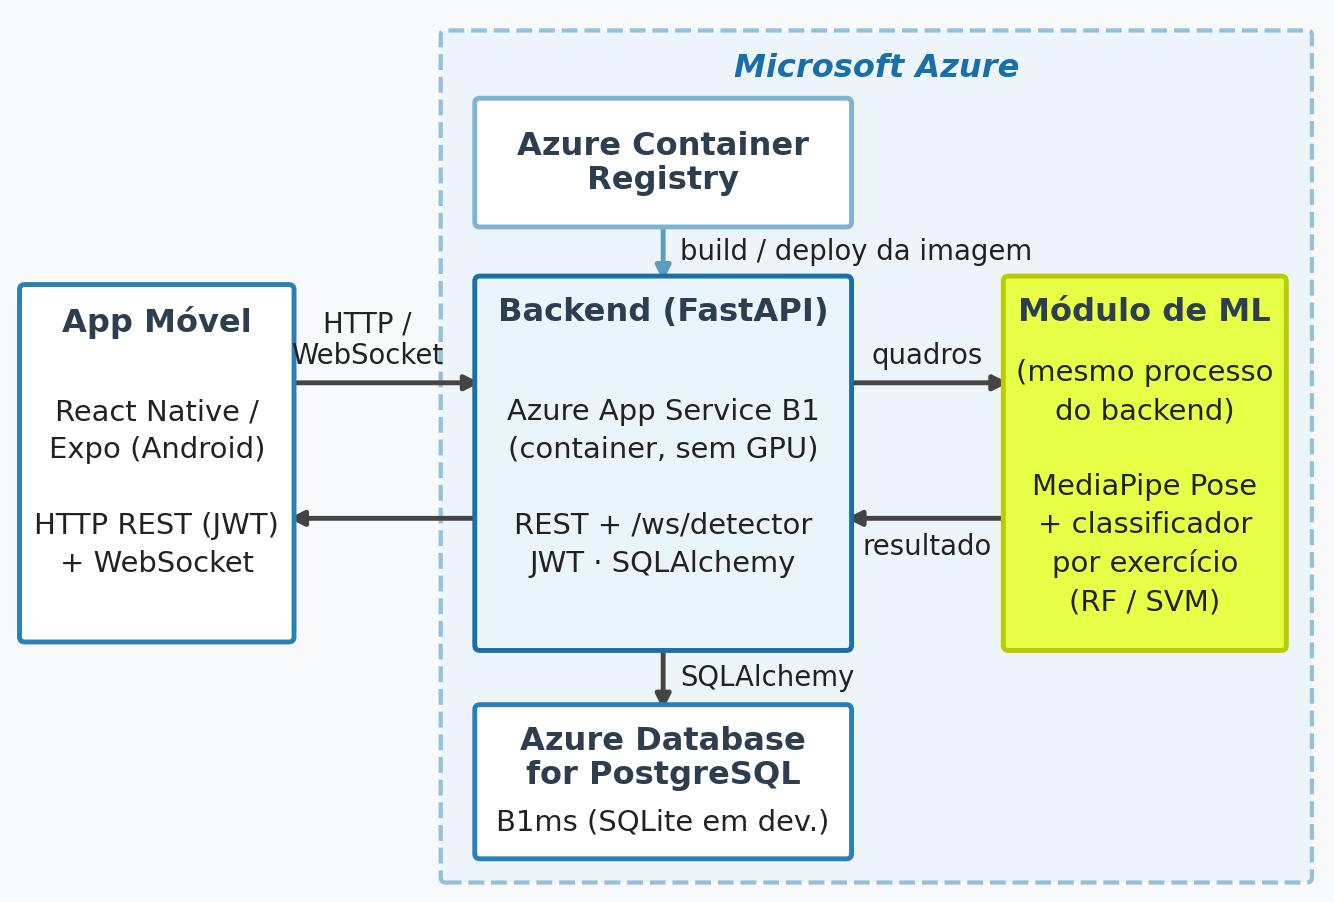
\includegraphics[width=.95\textwidth]{diagrama_arquitetura.jpg}
\caption{Diagrama de componentes do sistema e sua implantação em nuvem}
\label{fig:arquitetura}
\end{figure}
\FloatBarrier

\subsection{Aplicativo Móvel}

O cliente é um aplicativo React Native~\cite{reactnative} construído sobre
o \textit{framework} Expo~\cite{expo}, o que permite gerar builds nativas
para Android (e, potencialmente, iOS) a partir de uma única base de código
em JavaScript. O aplicativo oferece: autenticação de usuário; cadastro de
exercícios e montagem de fichas de treino (com séries, repetições e carga
por exercício); execução de sessões de treino com cronômetro e estimativa
de calorias (heurística linear que multiplica o tempo de treino pelo peso
corporal do usuário por um fator fixo por gênero, sem base em tabela de
gasto metabólico por exercício); histórico e estatísticas mensais de
treino; e a tela do detector, onde o usuário grava ou seleciona um vídeo
para análise de execução. A Figura~\ref{fig:usecases} apresenta o diagrama
de casos de uso do sistema, detalhando essas interações do usuário com o
aplicativo.

\begin{figure}[ht]
\centering
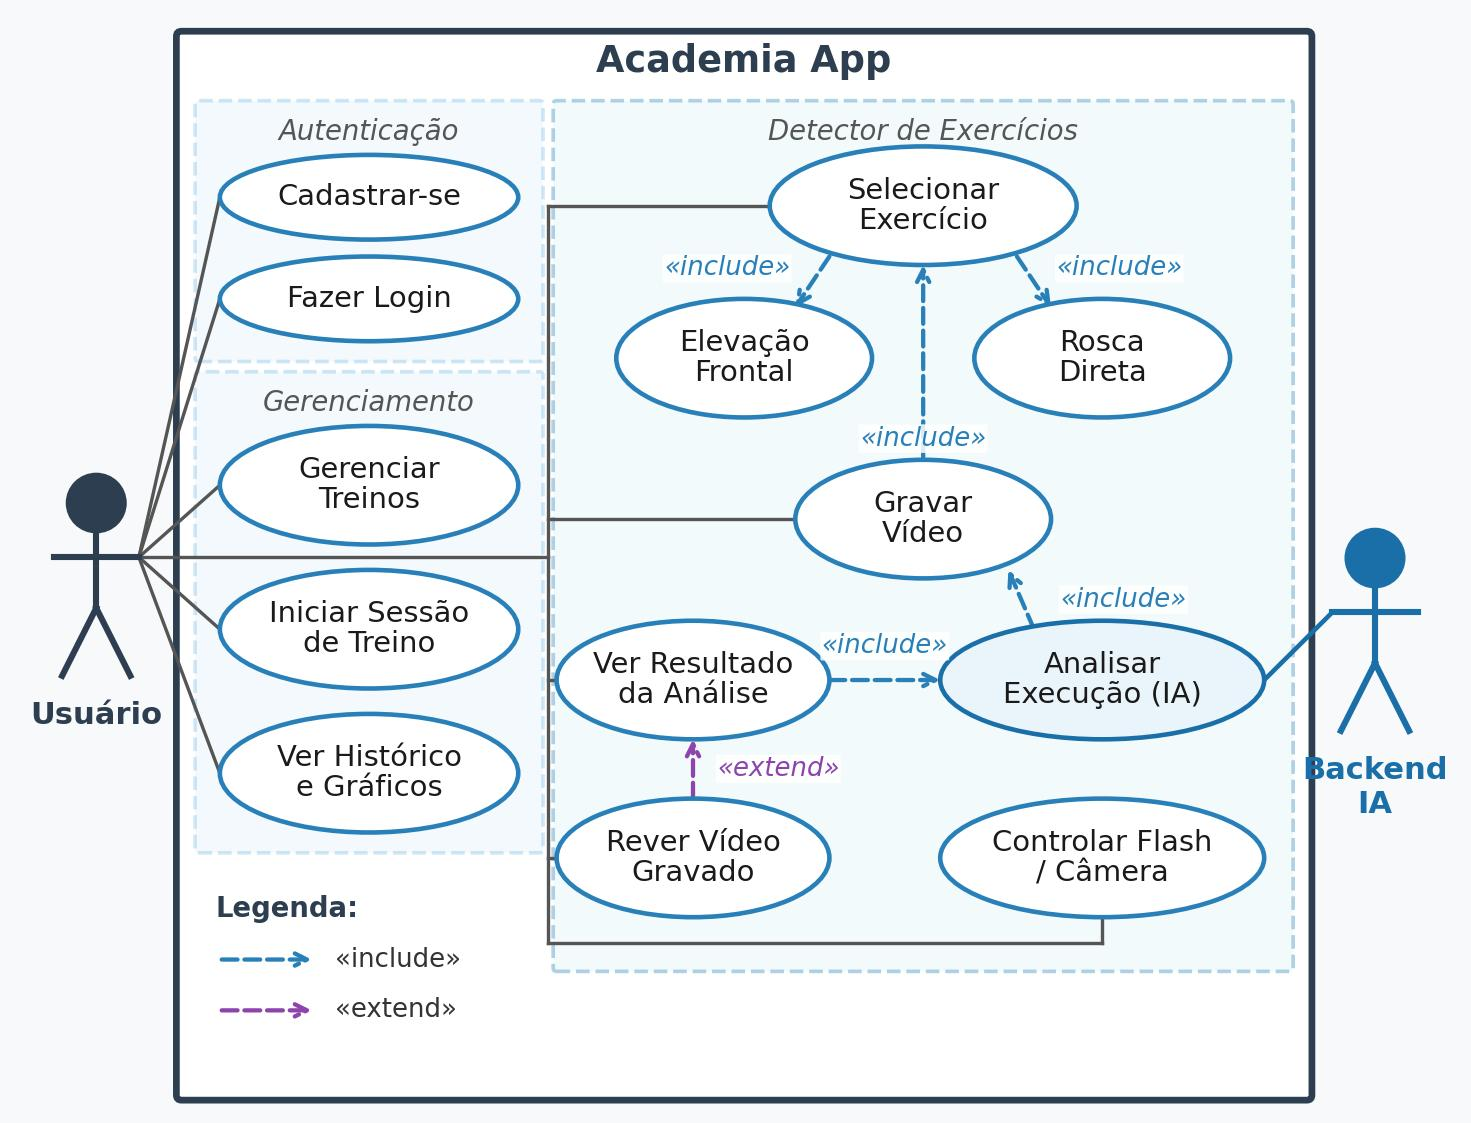
\includegraphics[width=.9\textwidth]{diagrama_use_cases.jpg}
\caption{Diagrama de casos de uso do sistema}
\label{fig:usecases}
\end{figure}
\FloatBarrier

A comunicação com o backend é feita via HTTP (API REST, com
\textit{token} JWT anexado a cada requisição) e, no caso do detector,
também via WebSocket para o modo de análise em tempo real (Seção~4.3).

\subsection{Backend}

O backend é implementado em Python com o \textit{framework}
FastAPI~\cite{fastapi}, escolhido pelo suporte nativo a rotas assíncronas
(relevante para o processamento de vídeo do detector, que é
computacionalmente custoso) e pela geração automática de documentação
interativa da API. A persistência de dados usa SQLAlchemy como ORM, com
SQLite em desenvolvimento local e PostgreSQL em produção (Seção~5); as
migrações de esquema são controladas com Alembic. A autenticação é feita
com \textit{tokens} JWT (biblioteca \texttt{python-jose}) e as senhas são
armazenadas com \textit{hash} \texttt{bcrypt}.

O modelo de dados relacional cobre usuários, exercícios, treinos (com
ordem, séries, repetições e carga por exercício dentro de um treino) e
sessões de treino executadas, cada uma com o registro detalhado (peso e
repetições) por série efetivamente realizada -- permitindo que a carga
usada em uma sessão real difira da carga planejada na ficha.

\section{Detecção de Execução de Exercícios}

O módulo de detecção é o principal componente de contribuição técnica
deste trabalho. Ele recebe um vídeo (gravado na hora ou selecionado da
galeria do usuário) e retorna, para cada repetição identificada, uma
classificação de "correta" ou "incorreta", com o nível de confiança do
modelo.

\subsection{Estimativa de Pose e Extração de Características}

Cada quadro do vídeo é processado com o MediaPipe
Pose~\cite{lugaresi2019mediapipe}, via a interface OpenCV~\cite{bradski2000opencv}
para leitura do vídeo, que estima a posição 2D de 33 pontos-chave (\textit{landmarks})
do corpo do praticante. A partir desses pontos são calculados ângulos
articulares (por exemplo, ângulo do braço em relação ao tronco e ângulo do
cotovelo, via arco-tangente das coordenadas dos três pontos que formam
cada articulação) e alturas relativas do punho em relação ao ombro,
normalizadas pela distância ombro--quadril do próprio usuário no vídeo --
o que torna as características robustas a diferenças de distância da
câmera e de proporção corporal entre usuários.

Cada exercício suportado define seu próprio conjunto de características e
sua própria regra de detecção de "repouso" (o instante em que o braço está
na posição inicial, usado para delimitar o início e o fim de cada
repetição). Atualmente o sistema suporta dois exercícios: Elevação Frontal
(\textit{front raise}), com 7 características (ângulo do braço e do
cotovelo de cada lado, altura relativa de cada punho e assimetria entre os
dois braços); e Rosca Bíceps, com 3 características (ângulo do cotovelo,
ângulo do braço e altura relativa do punho do lado com maior visibilidade
detectada pelo MediaPipe, para lidar com oclusão quando o exercício é
filmado de lado).

\subsection{Classificação Supervisionada por Exercício}

Na inferência, para cada repetição identificada (sequência de quadros
entre dois instantes de repouso, Seção~4.1), o sistema seleciona um único
quadro para classificar: o de maior valor, entre os quadros da repetição,
de uma métrica de intensidade específica do exercício -- para a elevação
frontal, o maior ângulo quadril--ombro--cotovelo entre os dois braços; para
a rosca bíceps, a maior flexão do cotovelo (180° menos o ângulo do
cotovelo). Formalmente, sendo $i_t$ essa métrica no quadro $t$ da
repetição, o quadro classificado é $\arg\max_t i_t$ -- o quadro de pico. O
classificador binário (correto/incorreto), implementado com
scikit-learn~\cite{pedregosa2011scikit} e treinado especificamente para
aquele exercício, é aplicado somente às características extraídas desse
quadro. O treinamento, descrito a seguir, não usa essa noção de pico: como
detalhado na Seção~6, cada quadro válido do dataset vira uma amostra de
treino independente, sem segmentação em repetições nem seleção de um
quadro representativo por repetição -- assimetria entre a amostragem de
treino e a amostragem de inferência discutida na Seção~7.1. Para a
elevação frontal, foi usado um classificador
Random Forest~\cite{breiman2001random} fixo, escolhido por seu bom
desempenho com conjuntos de características pequenos e de baixa
dimensionalidade (3 a 7 variáveis neste caso), por não exigir grande
volume de dados de treino em comparação a abordagens baseadas em redes
neurais profundas, e por permitir inspecionar a importância de cada
característica na decisão do modelo. Para a rosca bíceps, o processo de
treino compara três algoritmos -- Random Forest, Gradient Boosting e
SVM~\cite{cortes1995svm} -- cada um com busca de hiperparâmetros via
validação cruzada (5-fold, otimizando F1 macro), e seleciona
automaticamente o de melhor desempenho; na versão atual do modelo, o
selecionado foi um SVM com kernel RBF.

Os modelos foram treinados sobre o dataset de poses do projeto Pose
Trainer~\cite{chen2020posetrainerrepo} (Seção~2), com sequências de
elevação frontal e rosca bíceps extraídas via OpenPose (formato BODY\_18) e
rotuladas como "execução correta" ou "execução incorreta" (com erros de
forma como flexão do cotovelo na elevação frontal ou uso de momento do
corpo na rosca bíceps). A Tabela~\ref{tab:dataset} resume o volume de
dados usado no treinamento de cada modelo.

\begin{table}[ht]
\centering
\caption{Volume de dados de treino por exercício (dataset de
\cite{chen2020posetrainerrepo})}
\label{tab:dataset}
\begin{tabular}{lccc}
\hline
\textbf{Exercício} & \textbf{Vídeos (bom/ruim)} & \textbf{Amostras (linhas)} & \textbf{Correto/Incorreto} \\
\hline
Elevação Frontal & 15 / 13 & 626 & 343 / 283 \\
Rosca Bíceps     & 6 / 10  & 1158 & 465 / 693 \\
\hline
\end{tabular}
\end{table}

Cada vídeo de treino gera várias linhas de dados (uma por quadro válido
dentro de uma repetição, após filtro de confiança de detecção do
OpenPose), o que explica o número de amostras ser bem maior do que o
número de vídeos do dataset original.

\subsection{Pipeline de Análise: Vídeo Gravado vs. Tempo Real}

O sistema oferece dois modos de análise. O modo principal, usado pela
tela de detector do aplicativo, é a \textbf{análise de vídeo}: o usuário
grava (ou seleciona) um vídeo completo, que é enviado por
\textit{multipart/form-data} ao endpoint \texttt{POST /detector/analyze};
o backend processa o vídeo quadro a quadro (descartando quadros conforme
uma taxa de amostragem fixa, para reduzir custo computacional sem perda
perceptível de qualidade de detecção) e retorna a lista de repetições
classificadas de uma só vez. Esse modo foi adotado após uma primeira
versão baseada em \textit{streaming} de quadros por WebSocket em tempo
real ter se mostrado pouco confiável em rede móvel real -- observação
empírica feita durante os testes de desenvolvimento, sem metodologia
formal de medição, mas com a taxa efetiva de quadros processados por
segundo caindo, em uso na rede móvel, para uma ordem de grandeza
claramente insuficiente para capturar o pico de movimentos rápidos -- o
endpoint WebSocket (\texttt{/ws/detector}) foi mantido no
backend por compatibilidade, mas o fluxo principal do aplicativo usa o
modo de vídeo gravado.

Como otimização de desempenho, vídeos com resolução muito alta (por
exemplo, 4K gravado pela câmera nativa do celular) têm cada quadro
redimensionado antes de passar pelo MediaPipe, e a leitura do vídeo evita
decodificar quadros que seriam descartados pela taxa de amostragem,
reduzindo o tempo de processamento sem alterar o resultado da
classificação.

\subsection{Privacidade e Retenção de Dados}

O módulo de detecção envia, do celular do usuário ao backend, um vídeo no
qual a pessoa que está treinando é identificável -- dado pessoal sensível
sob a Lei Geral de Proteção de Dados (LGPD, Lei 13.709/2018). O tratamento
implementado, porém, é efêmero: o vídeo recebido é gravado em um arquivo
temporário do sistema operacional do servidor, processado quadro a quadro,
e removido assim que a análise termina, dentro de um bloco de finalização
executado mesmo em caso de erro durante o processamento -- não há gravação
em disco persistente, banco de dados ou armazenamento de objetos
(\textit{blob storage}) na Azure. Também não há persistência do resultado
da classificação: o backend devolve, na própria resposta HTTP, apenas os
derivados numéricos da análise (número de repetições, classificação e
confiança por repetição), que o aplicativo exibe ao usuário mas não
reenvia ao servidor para armazenamento. Essa arquitetura reduz a
superfície de exposição de dados pessoais sensíveis, mas a implementação
atual não inclui uma tela de consentimento explícito informando ao
usuário, antes do envio, que o vídeo será transmitido a um servidor remoto
para processamento -- uma lacuna sob a ótica de finalidade e transparência
exigidas pela LGPD, ainda que o dado, uma vez recebido, não seja retido.

\section{Implantação em Nuvem}

Para validar o sistema fora do ambiente de desenvolvimento local, o
backend foi conteinerizado com Docker~\cite{docker} e implantado na
Microsoft Azure, usando Azure Container Registry para armazenar a imagem,
Azure App Service (camada B1) para executar o container e Azure Database
for PostgreSQL (camada B1ms) para persistência -- substituindo o SQLite
usado em desenvolvimento local. O aplicativo móvel foi então compilado
como um pacote Android autônomo (\textit{build} EAS, perfil
\textit{preview}), já apontando para o backend hospedado na nuvem, sem
depender de um servidor de desenvolvimento (\textit{Metro}) local.

\section{Metodologia de Avaliação}

Esta seção descreve o protocolo efetivamente usado para treinar e avaliar
os classificadores de execução (Seção~4.2), antes de os resultados serem
apresentados na Seção~7.

Os dados de treino têm origem no dataset público do projeto Pose
Trainer~\cite{chen2020posetrainerrepo} (Seção~2.3): sequências de pose,
extraídas com OpenPose (formato BODY\_18) a partir de vídeos de execuções
de elevação frontal e rosca bíceps, rotuladas por vídeo como "correta" ou
"incorreta". Um script de geração de dataset processa cada vídeo quadro a
quadro, descarta os quadros em posição de repouso e os de baixa confiança
de detecção, calcula os ângulos articulares de cada quadro remanescente e
grava cada um como uma linha independente de um arquivo CSV -- sem
preservar qualquer identificador do vídeo ou do usuário de origem daquele
quadro. A Tabela~\ref{tab:dataset} (Seção~4.2) resume o volume resultante:
626 linhas a partir de 28 vídeos para elevação frontal, e 1158 linhas a
partir de 16 vídeos para rosca bíceps.

O particionamento treino/teste (80\%/20\%) e os \textit{folds} da
validação cruzada 5-fold são feitos sobre essas linhas, ou seja, por
quadro, e não por vídeo: como o identificador do vídeo de origem não é
preservado no CSV, não é possível, nem no código nem a posteriori, garantir
ou mesmo verificar que os quadros de um mesmo vídeo caiam inteiramente do
mesmo lado da partição. Como quadros consecutivos de uma mesma repetição
tendem a ser muito semelhantes entre si, é provável que quadros de um
mesmo vídeo apareçam tanto no conjunto de treino quanto no de teste (ou em
\textit{folds} diferentes da validação cruzada). As consequências dessa
limitação do protocolo de avaliação para a leitura das métricas reportadas
são discutidas na Seção~7.1.

As métricas reportadas na Seção~7 são: acurácia no conjunto de teste (20\%
dos dados, não usado no treino) e acurácia média $\pm$ desvio-padrão em
validação cruzada 5-fold, para a elevação frontal; e acurácia no conjunto
de teste e F1 macro em validação cruzada 5-fold, para a rosca bíceps --
métrica usada também como critério de seleção entre os três algoritmos
candidatos (Random Forest, Gradient Boosting e SVM) via busca de
hiperparâmetros. Não foram calculadas matriz de confusão nem métricas por
classe (precisão e revocação individuais) para nenhum dos dois modelos,
lacuna também discutida na Seção~7.1.

\section{Resultados e Discussão}

O sistema completo -- cadastro, montagem e execução de treinos, histórico
de sessões e detector de exercícios -- está implantado e funcional, com o
backend hospedado na Azure e testado a partir de um \textit{build} Android
real, fora do ambiente de desenvolvimento. Os dois classificadores
atingiram, no conjunto de teste separado (20\% dos dados, não usado no
treino), acurácia de 79\% para a elevação frontal (Random Forest, com
acurácia por validação cruzada de 5-fold de 83\% $\pm$ 3\%) e 85\% para a
rosca bíceps (SVM com kernel RBF, selecionado por validação cruzada entre
Random Forest, Gradient Boosting e SVM, com F1 macro de 0,85).

\subsection{Limitações Identificadas}

As acurácias reportadas acima (79\% e 85\%) devem ser lidas com uma
ressalva sobre o protocolo de avaliação, descrito na Seção~6: como o
particionamento treino/teste e os \textit{folds} da validação cruzada são
feitos por quadro, sobre 626 quadros de 28 vídeos (elevação frontal) e
1158 quadros de 16 vídeos (rosca bíceps), e como o identificador do vídeo
de origem não é preservado no dataset, quadros de um mesmo vídeo -- e
portanto quase-duplicatas de uma mesma repetição -- provavelmente aparecem
tanto no treino quanto no teste. Essas métricas devem, portanto, ser lidas
como um limite superior otimista do desempenho do classificador, e não
como uma medida de generalização para um usuário ou vídeo nunca visto pelo
modelo. Reavaliar os dois classificadores com particionamento por vídeo
(por exemplo, \texttt{GroupKFold}, agrupando quadros pelo vídeo de origem)
é um item de trabalho futuro (Seção~8).

A principal limitação identificada durante os testes com execuções reais
do usuário -- e, como se argumenta a seguir, também a mais diretamente
explicável a partir do próprio desenho do pipeline de treino e inferência
-- é que o modelo permanece preso ao estilo em que o dataset de treino foi
filmado. Essa limitação tem um mecanismo causal específico: como descrito
na Seção~4.2, a inferência classifica sempre o quadro de pico da
repetição (o de maior ângulo de braço, no caso da elevação frontal),
enquanto o treino, ao contrário da inferência, não seleciona um quadro de
pico por repetição -- todo quadro não-repouso do vídeo vira uma amostra
independente, sem qualquer preferência por quadros de maior amplitude
(Seção~6). O quadro que o classificador de fato vê em produção -- o pico,
por construção o de maior ângulo da repetição -- é justamente aquele para
o qual o treino tem menos e menos representativa cobertura: o dataset
nunca passa de aproximadamente 110° de ângulo do braço e 35° de assimetria
entre os dois braços, enquanto execuções reais dos usuários -- inclusive
tecnicamente corretas -- chegam a 172° e 97°, bem além do que o modelo já
viu como exemplo, faixa em que o classificador tende a extrapolar mal e
produzir classificações instáveis. Ou seja, o descasamento entre a
amostragem de treino (todo quadro válido, sem segmentação em repetições) e
a amostragem de inferência (um único quadro, sempre o de maior amplitude
da repetição) não é só uma inconsistência de engenharia: é o mecanismo que
faz o classificador operar, em uso real, sistematicamente fora do suporte
dos dados em que foi treinado.

Além da amplitude do movimento, uma observação preliminar aponta na mesma
direção quanto à forma como o vídeo é filmado: em testes repetidos, para
os dois exercícios, sempre que uma segunda pessoa grava a execução do
autor deste trabalho (segurando o celular, tipicamente numa altura e
ângulo mais próximos dos olhos, acompanhando o movimento) o modelo
classifica errado; quando o autor se grava, com a câmera fixa em algum
apoio e normalmente numa altura mais baixa, a classificação funciona
corretamente. Essa observação não constitui um experimento controlado --
não há registro sistemático de taxa de erro por posição de câmera, e o
único sujeito testado foi o próprio autor --, mas é consistente com a
mesma causa raiz: o dataset reaproveitado de
terceiros~\cite{chen2020posetrainerrepo} foi filmado num estilo específico
de posicionamento de câmera, e o ângulo de projeção 2D de uma mesma
execução muda conforme a câmera muda de posição. Um experimento
controlado -- mesma execução repetida em três posições de câmera, com taxa
de erro de classificação medida por posição -- é proposto como trabalho
futuro (Seção~8) para isolar esse fator da amplitude de movimento.

Dois outros descasamentos entre o pipeline de treino e o de inferência
foram identificados por inspeção direta do código, e ainda não têm seu
impacto isolado experimentalmente. O primeiro é o já mencionado
(Seção~2.2): o pipeline de extração de pose usado na produção (MediaPipe)
difere do pipeline usado para gerar o dataset (OpenPose), estimadores que
não produzem exatamente os mesmos valores para as mesmas articulações. O
segundo é um descasamento no critério de repouso da rosca bíceps: o script
que curou o dataset descarta como repouso quadros com ângulo de cotovelo
acima de 155°, enquanto a inferência em produção considera repouso a
partir de 130° -- ou seja, quadros com o cotovelo entre 130° e 155° foram
incluídos no treino como exemplos válidos de execução, mas em produção
esses mesmos quadros já seriam tratados como repouso e nunca chegariam a
ser o quadro de pico de uma repetição (para a elevação frontal os dois
limiares coincidem, em 20°). A unificação desses limiares é proposta como
trabalho futuro (Seção~8). Por ter sido coletado para outro projeto, o
dataset reaproveitado também não foi desenhado especificamente em torno da
variabilidade de execução dos usuários deste aplicativo -- nem de
amplitude de movimento, nem de posicionamento de câmera.

A avaliação dos dois classificadores também se limitou a métricas
agregadas: acurácia no conjunto de teste e em validação cruzada para os
dois exercícios, e F1 macro em validação cruzada para a rosca bíceps
(Seção~6) -- sem matriz de confusão nem métricas por classe (precisão e
revocação individuais para "correto" e "incorreto"). Essa lacuna importa
em particular num detector de execução, em que os dois tipos de erro têm
custo assimétrico: classificar como correta uma repetição na verdade
incorreta pode reforçar no usuário um padrão de movimento lesivo, um custo
maior do que o de classificar como incorreta uma repetição na verdade
correta. O dataset da rosca bíceps também é desbalanceado (465 quadros
"correto" contra 693 "incorreto", Tabela~\ref{tab:dataset}), o que pode
enviesar o classificador na direção da classe majoritária sem que isso
apareça na acurácia agregada. Calcular precisão e revocação por classe
para os dois modelos é proposto como trabalho futuro (Seção~8).

Por fim, a detecção do estado de repouso (Seção~4.1), da qual depende toda
a segmentação de um vídeo em repetições e, por consequência, toda a
classificação, não foi avaliada isoladamente -- não há medição de quantas
repetições reais são corretamente detectadas, perdidas (fundidas com a
repetição seguinte) ou criadas espuriamente (uma única repetição dividida
em duas). Um protocolo para essa avaliação -- vídeos com número de
repetições conhecido a priori, comparando contra o número de repetições
detectadas, perdidas e falsas -- é proposto como trabalho futuro
(Seção~8).

A superação da limitação de amplitude e posicionamento de câmera depende de ampliar o conjunto de treino com
vídeos próprios que cubram tanto a faixa de amplitude alta (exemplos
corretos, incluindo a leve dessincronia natural entre os dois braços que
ocorre em execuções reais, e exemplos incorretos na mesma faixa) quanto
variações realistas de posicionamento de câmera (gravação por terceiros,
alturas e ângulos diferentes), para que o modelo aprenda a generalizar
além do estilo específico do dataset original, em vez de associar
qualquer desvio desse estilo a um erro de execução.

\section{Conclusão e Trabalhos Futuros}

Este trabalho apresentou o desenvolvimento de um aplicativo móvel de
gerenciamento de treinos com um módulo de detecção da qualidade de
execução de exercícios baseado em estimativa de pose e aprendizado de
máquina supervisionado, cobrindo desde a arquitetura do sistema até sua
implantação em um ambiente de nuvem real. O processo de desenvolvimento
evidenciou que, em um sistema desse tipo, os principais riscos técnicos
não estão apenas na escolha do algoritmo de classificação, mas também na
representatividade do conjunto de dados de treino frente à variabilidade
real de execução dos usuários.

Como trabalhos futuros, destacam-se: (i) a ampliação do conjunto de
dados de treino com vídeos próprios, cobrindo tanto a faixa de amplitude
de movimento quanto a variação de posicionamento de câmera identificadas
como deficientes no dataset de terceiros atualmente reaproveitado; (ii) a
criação de uma
ferramenta de extração de dataset diretamente a partir do MediaPipe,
substituindo o pipeline OpenPose herdado do dataset original e unificando
o estimador de pose usado em treino e em produção; (iii) a adição de novos
exercícios ao detector, reaproveitando o pipeline de extração de
características e classificação já estabelecido; e (iv) a validação de
usabilidade do detector com um grupo maior de usuários reais, fora do
próprio autor do trabalho.

\bibliographystyle{sbc}
\bibliography{referencias}

\end{document}
